\documentclass[a4paper, 14pt]{extarticle}
\usepackage[russian]{babel}
\usepackage[T1]{fontenc}
\usepackage{fontspec}
\usepackage{indentfirst}
\usepackage{enumitem}
\usepackage{graphicx}
\usepackage[
  left=20mm,
  right=10mm,
  top=20mm,
  bottom=20mm
]{geometry}
\usepackage{parskip}
\usepackage{titlesec}
\usepackage{xurl}
\usepackage{hyperref}
\usepackage{float}
\usepackage[
  figurename=Рисунок,
  labelsep=endash,
]{caption}
\usepackage[outputdir=build, newfloat]{minted}

\hypersetup{
  colorlinks=true,
  linkcolor=black,
  filecolor=blue,
  urlcolor=blue,
}

\renewcommand*{\labelitemi}{---}
\setmainfont{Times New Roman}
\setmonofont{JetBrains Mono}[
  SizeFeatures={Size=11},
]

\newenvironment{code}{\captionsetup{type=listing}}{}
\SetupFloatingEnvironment{listing}{name=Листинг}

\setminted{
  fontsize=\footnotesize,
  frame=lines,
  framesep=2mm,
}

\setlength{\parskip}{6pt}

\setlength{\parindent}{1cm}
\setlist[itemize]{itemsep=0em,topsep=0em,parsep=0em,partopsep=0em,leftmargin=2.0cm,wide}
\setlist[enumerate]{itemsep=0em,topsep=0em,parsep=0em,partopsep=0em,leftmargin=2.0cm,wide}

\renewcommand{\thesection}{\arabic{section}.}
\renewcommand{\thesubsection}{\thesection\arabic{subsection}.}
\renewcommand{\thesubsubsection}{\thesubsection\arabic{subsubsection}.}

\titleformat{\section}{\normalfont\bfseries}{\thesection}{0.5em}{}
\titleformat{\subsection}{\normalfont\bfseries}{\thesubsection}{0.5em}{}

\titleformat*{\section}{\normalfont\bfseries}
\titleformat*{\subsection}{\normalfont\bfseries}

\linespread{1.5}
\renewcommand{\baselinestretch}{1.5}

\begin{document}

\begin{titlepage}
  \vspace{0pt plus2fill}
  \noindent

  \vspace{0pt plus6fill}
  \begin{center}
    Санкт-Петербургский национальный исследовательский университет
    информационных технологий, механики и оптики

    \vspace{0pt plus3fill}

    Факультет инфокоммуникационных технологий

    Направление подготовки 11.03.02

    \vspace{0pt plus2fill}

    Лабораторная работа №1

    <<Введение в web-разработку>>

  \end{center}

  \vspace{0pt plus9fill}
  \begin{flushright}
    Выполнил: \\
    Швалов Даниил Андреевич

    Группа: К33211

    Проверила: \\
    Марченко Елена Вадимовна
  \end{flushright}

  \vspace{0pt plus2fill}
  \begin{center}
    Санкт-Петербург

    2023
  \end{center}
\end{titlepage}

\section{Введение}

\textbf{Цель работы}: научиться создавать web-страницы, использующие HTML,
стили CSS и код JavaScript.

\section{Ход работы}

\subsection{Упражнение №1}

В результате выполнения упражнения был получен код, представленный в листинге
\ref{code:sample-01}.

\begin{code}
  \label{code:sample-01}
  \inputminted{html}{../task-1/Sample01.html}
  \caption{Итоговый исходный код упражнения №1}
\end{code}

В данном исходном коде были использованы следующие тэги:
\begin{itemize}
  \item \texttt{html} --- корневой элемент HTML-документа. Сообщает браузеру,
  что это HTML-документ. Является контейнером для всех остальных
  html-элементов.
  \item \texttt{head} --- элемент-контейнер для метаданных HTML-документа,
  таких как \texttt{<title>}, \texttt{<meta>}, \texttt{<script>},
  \texttt{<link>}, \texttt{<style>}.
  \item \texttt{meta} --- используется для хранения дополнительной информации о
  странице. Эту информацию используют браузеры при обработке страницы, а
  поисковые системы — для ее индексации. В блоке \texttt{<head>} может
  быть несколько элементов \texttt{<meta>}, так как в зависимости от
  используемых атрибутов они несут разную информацию.
  \item \texttt{title} --- заголовок HTML-документа, отображаемый в верхней
  части строки заголовка браузера.
  \item \texttt{body} --- представляет тело документа, т. е. содержимое, не
  относящееся к метаданным документа.
  \item \texttt{h1} --- заголовок первого уровня.
  \item \texttt{p} --- абзац текста.
\end{itemize}

Веб-страница, которая получилась при выполнении упражнения, показана на рис.
\ref{fig:task-1}.

\begin{figure}[H]
  \centering
  \fbox{
\includegraphics[width=0.5\textwidth]{images/task-1.png}}
  \caption{Итоговый вид получившейся веб-страницы}
  \label{fig:task-1}
\end{figure}

\subsection{Упражнение №2}

В данном упражнении в код страницы был добавлен тэг \texttt{style} и заданы
цвет страницы и цвет параграфа. Итоговый исходный код находится в листинге
\ref{code:task-2}.

\begin{code}
  \label{code:task-2}
  \inputminted{html}{../task-2/Sample02.html}
  \caption{Итоговый исходный код упражнения №2}
\end{code}

Тэг \texttt{style} используется для того, чтобы подключить встраиваемые таблицы
стилей.

Веб-страница, которая получилась при выполнении упражнения, показана на рис.
\ref{fig:task-2}.

\begin{figure}[H]
  \centering
  
\includegraphics[width=0.5\textwidth]{images/task-2.png}
  \caption{Итоговый вид получившейся веб-страницы}
  \label{fig:task-2}
\end{figure}

\subsection{Упражнение №3}

В данном упражнении в код страницы был добавлен тэг \texttt{script}, а также
вызов функции \texttt{alert}, который отображает сообщение со строкой <<Привет
мир!>>. Итоговый исходный код находится в листинге \ref{code:task-3}.

\begin{code}
  \label{code:task-3}
  \inputminted{html}{../task-3/Sample03.html}
  \caption{Итоговый исходный код упражнения №3}
\end{code}

Тэг \texttt{script} используется для того, чтобы определить сценарий на стороне
клиента на JavaScript. Содержит либо текст скрипта, либо указывает на внешний
файл сценария с помощью атрибута \texttt{src}.

Функция \texttt{alert} используется для того, чтобы вывести на экран окно с
сообщением.

Веб-страница, которая получилась при выполнении упражнения, показана на рис.
\ref{fig:task-3}.

\begin{figure}[H]
  \centering
  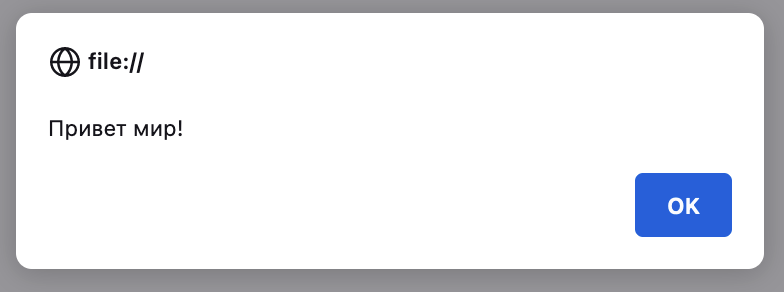
\includegraphics[width=0.5\textwidth]{images/task-3.png}
  \caption{Итоговый вид получившейся веб-страницы}
  \label{fig:task-3}
\end{figure}

\section{Вывод}

В ходе выполнения лабораторной работы и выполнения упражнений я научился
создавать web-страницы, использующие HTML, стили и код JavaScript.

\section{Ответы на вопросы}

\begin{enumerate}[leftmargin=*]
  \item Какие объекты могут содержаться внутри документа HTML?

  \textbf{Ответ}: внутри HTML документа могут содержаться тэги (парные и
  непарные), с помощью которых можно добавлять и форматировать элементы
  документа.
  \item Чем отличаются парные и непарные теги?

  \textbf{Ответ}: Парные теги состоят из двух частей --- открывающего и
  закрывающего тегов. Открывающий тег обозначается как и одиночный ---
  \texttt{<тег>}, а в закрывающем используют слеш --- \texttt{</тег>}
  (например, \texttt{<html>} \ldots \texttt{</html>}). Парные теги могут
  быть вложенными.

  Непарные тэги состоят только из одного тэга (например, \texttt{<meta>}
  или \texttt{<br>}). Также перед закрывающей скобкой можно использовать
  слеш (например, \texttt{<meta/>} или \texttt{<br/>})
  \item Основные правила записи тегов и их атрибутов.

  \textbf{Ответ}: Теги должны должны быть строго вложенными друг в друга.
  Например, \texttt{<a><b></b></a>} --- корректная конструкция, а
  \texttt{<a><b></a></b>} --- некорректная.

  Атрибуты могут быть только в открывающем теге, их может быть несколько,
  разделяются они пробелами.
  \item Какие теги определяют служебную и содержательную области документа
  HTML?

  \textbf{Ответ}: HTML-документы состоят из двух разделов: заголовка,
  который задается парным тегом \texttt{<head>}, и основного раздела,
  задающегося парным тегом \texttt{<body>}. Они являются обязательными
  для всех HTML-документов.
  \item Для чего служит тег \texttt{<img>}? Почему атрибут \texttt{src} этого
  тега является обязательным?

  \textbf{Ответ}: Тег \texttt{<img>} встраивает изображение в документ.
  Атрибут \texttt{src} обязателен и содержит путь к изображению, которое
  необходимо встроить в документ. Также тег \texttt{<img>} может
  принимать атрибут \texttt{alt}, который содержит текстовое описание
  изображения.
  \item META-теги и их атрибуты. Приведите примеры значений атрибутов
  МЕТА-тегов.

  \textbf{Ответ}: Мета-теги используются для указания метаданных. Элемент
  \texttt{<meta>} включает в себя следующие атрибуты:
  \begin{itemize}
    \item \texttt{charset} --- задаёт кодировку символов, используемую на
    страниц (например, \texttt{utf-8});
    \item \texttt{http-equiv} --- задает значение, которое совместно с
    атрибутом \texttt{content}, будет преобразовано в формат
    заголовка ответа HTTP. Браузер обрабатывает эти заголовки так,
    как будто они прибыли непосредственно от сервера. Примерами
    таких значений могут быть \texttt{content-type},
    \texttt{set-cookie} и др.
    \item \texttt{content} --- содержит значение для атрибута
    \texttt{http-equiv} или атрибута \texttt{name};
    \item \texttt{name} --- устанавливает идентификатор мета-тега для
    пары имя=значение. Одновременно использовать атрибуты \texttt{name}
    и \texttt{http-equiv} не допускается. Может принимать такие
    значения, как \texttt{author}, \texttt{description},
    \texttt{keywords} и др.
  \end{itemize}
\end{enumerate}

\end{document}
